\documentclass{ximera}


\graphicspath{
  {./}
  {ximeraTutorial/}
  {basicPhilosophy/}
}

\newcommand{\mooculus}{\textsf{\textbf{MOOC}\textnormal{\textsf{ULUS}}}}

\usepackage{tkz-euclide}\usepackage{tikz}
\usepackage{tikz-cd}
\usetikzlibrary{arrows}
\tikzset{>=stealth,commutative diagrams/.cd,
  arrow style=tikz,diagrams={>=stealth}} %% cool arrow head
\tikzset{shorten <>/.style={ shorten >=#1, shorten <=#1 } } %% allows shorter vectors

\usetikzlibrary{backgrounds} %% for boxes around graphs
\usetikzlibrary{shapes,positioning}  %% Clouds and stars
\usetikzlibrary{matrix} %% for matrix
\usepgfplotslibrary{polar} %% for polar plots
\usepgfplotslibrary{fillbetween} %% to shade area between curves in TikZ
\usetkzobj{all}
\usepackage[makeroom]{cancel} %% for strike outs
%\usepackage{mathtools} %% for pretty underbrace % Breaks Ximera
%\usepackage{multicol}
\usepackage{pgffor} %% required for integral for loops



%% http://tex.stackexchange.com/questions/66490/drawing-a-tikz-arc-specifying-the-center
%% Draws beach ball
\tikzset{pics/carc/.style args={#1:#2:#3}{code={\draw[pic actions] (#1:#3) arc(#1:#2:#3);}}}



\usepackage{array}
\setlength{\extrarowheight}{+.1cm}
\newdimen\digitwidth
\settowidth\digitwidth{9}
\def\divrule#1#2{
\noalign{\moveright#1\digitwidth
\vbox{\hrule width#2\digitwidth}}}






\DeclareMathOperator{\arccot}{arccot}
\DeclareMathOperator{\arcsec}{arcsec}
\DeclareMathOperator{\arccsc}{arccsc}

















%%This is to help with formatting on future title pages.
\newenvironment{sectionOutcomes}{}{}


\title{Angles}

\begin{document}

\begin{abstract}
elevation and depression
\end{abstract}
\maketitle


We have other measurements, besides length, that might be changing in a situation.




\[
\text{rate} = \frac{\Delta \text{angle}}{\Delta \text{time}} 
\]

\textbf{Note:} $\Delta \text{angle}$ might be measured in degrees or radians. Calculus will use radians.\\






\subsection{Airplane}

An airplane is flying overhead on a level flight path, 5 miles above the ground.  The plane is travelling at a constant speed and will travel directly over a tracking station. The tracking station's radar antennea measures the distance from the station to the plane.







$\blacktriangleright$ We have two pertinent angles:

Angles $\alpha$ and $\beta$ both are functions of $t$: $\alpha(t)$ and $\beta(t)$.







An airplane is flying overhead on a level flight path, 5 miles above the ground.  The plane is travelling at a constant speed and will travel directly over a tracking station. The tracking station's radar antennea measures the distance from the station to the plane. If the distance between the station and the plane is decreasing at a rate of $350$ miles per hour when that distance is $10$ miles, then what is the speed of the plane?








\textbf{\textcolor{purple!85!blue}{Step 1: A Picture}}


\begin{image}
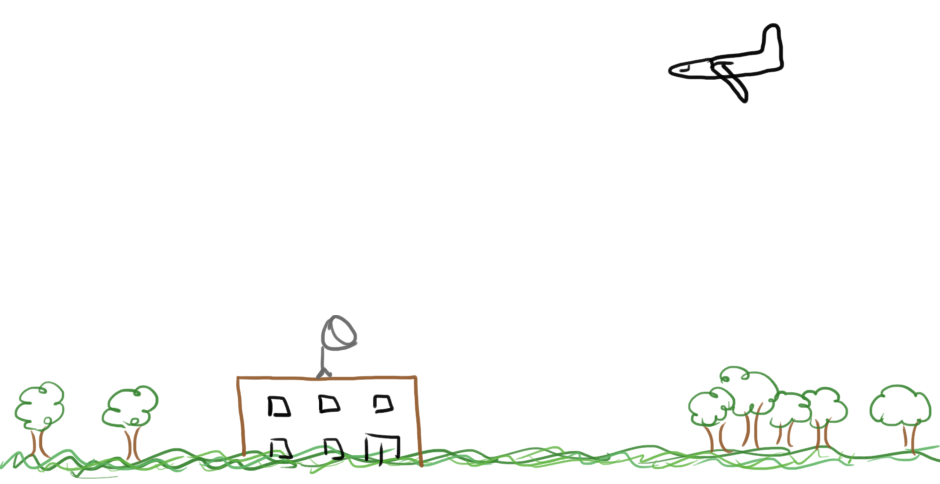
\includegraphics{pics/plane_1.png}
\end{image}




\textbf{\textcolor{purple!85!blue}{Step 2: Identify Measurements}}



\begin{image}
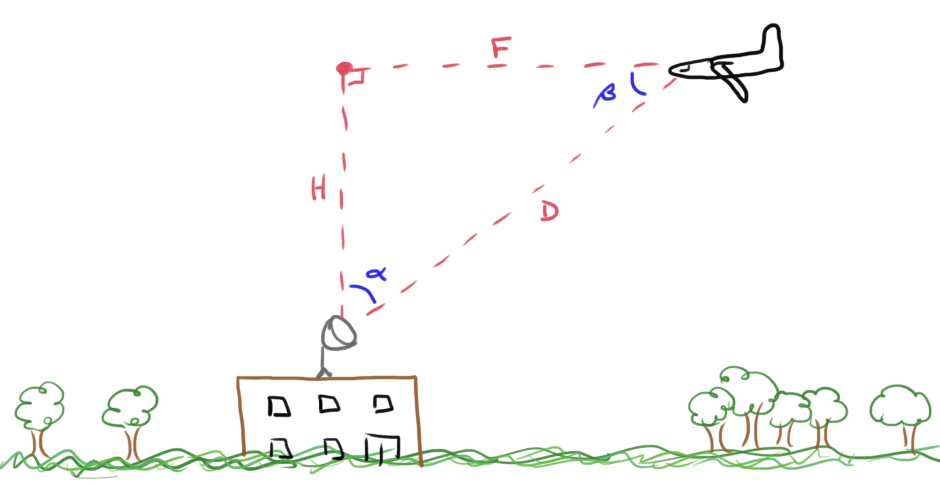
\includegraphics{pics/plane_3.png}
\end{image}



$\blacktriangleright$ We have two pertinent angles:

\begin{itemize}
\item $\alpha$ is the angle of elevation from the station to the plane.
\item $\beta$ is the angle of depression from the plane to the station.
\end{itemize}

Both of these are functions of time, $t$: $\alpha(t)$ and $\beta(t)$.






\begin{question} $\boxdot$ 

Is $\alpha(t)$ an increasing or decreasing function with respect to $t$?

\begin{multipleChoice}
\choice {Increasing}
\choice[correct] {Decreasing}
\end{multipleChoice}

\end{question}








\begin{question} $\boxdot$ 

Is $\beta(t)$ an increasing or decreasing function with respect to $t$?

\begin{multipleChoice}
\choice[correct] {Increasing}
\choice {Decreasing}
\end{multipleChoice}

\end{question}







These angles are related to the sides of the triangle through sine and cosine.










\begin{question} $\boxdot$ 

Which expression represents $\sin(\alpha)$?

\begin{multipleChoice}
\choice {$\frac{F}{H}$}
\choice {$\frac{D}{F}$}
\choice[correct] {$\frac{F}{D}$}
\choice {$\frac{H}{D}$}
\end{multipleChoice}

\end{question}









\begin{question} $\boxdot$ 

Which expression represents $\cos(\beta)$?

\begin{multipleChoice}
\choice {$\frac{F}{H}$}
\choice {$\frac{D}{F}$}
\choice[correct] {$\frac{F}{D}$}
\choice {$\frac{H}{D}$}
\end{multipleChoice}

\end{question}




















\end{document}
